\chapter{Task 46: EU transportation network II}
\section{Task Description}
The aim of this project is to build a network from raw geographical data of European railways.
\medskip \newline
The data used for the analysis is sourced from the \textit{EuroGlobalMap (EGM)} database, which is published under an open license by EuroGeographics. EuroGeographics is a not-for-profit membership association for European National Mapping, Cadastral, and Land Registration Authorities (NMCAs), in partnership with the National Geographic Institute (NGI) Belgium. The latest data is available at mapsforeurope.org. For this analysis, we refer to the EGM 2019 dataset, released in March 2019.
\medskip \newline
The requested output of Project \#46 consists of two \textbf{.csv} files for each country with an ISO3 code starting from IT onwards (in alphabetical order) and for the whole of Europe:
\begin{itemize}
    \item \textbf{country\_nodes.csv}, which shall contain the columns (nodeID, nodeLabel, latitude, longitude, country\_name, country\_ISO3). Node identifiers must be sequential integer numbers starting from $1$.
    \item \textbf{country\_edges.csv}, containing edges list with columns (nodeID\_from, nodeID\_to, node\_label\_from, node\_label\_to).
\end{itemize}
The choice of what exactly the nodes of the network should represent (cities, administrative districts, etc.) is not specifically prescribed. We decided to construct networks where \textbf{nodes are identified with cities} and \textbf{two cities are connected through an edge if and only if they are consecutive stops of some railway}. After some preliminary trials (and failures!), we discovered that the quickest and most effective method to build the city/rails network involves first creating an initial "raw" network. In this raw network, each straight segment of rails is represented as a pair of nodes connected by an edge. Subsequently, the city/rails network is built as a subset of this raw network. 
\medskip \newline
With this approach in mind, Section [1 - Data Extraction] is organized as follows:
\begin{itemize}
\item In Paragraph 1.1, we describe the method used to read the raw data from the EGM19 database and present a preliminary visualization of this data.
\item In Paragraph 1.2, we outline the main steps for creating the "raw" networks.
\item In Paragraph 1.3, we detail the main steps for constructing the city/rails network.
\end{itemize}
\noindent Section [$2$ - Results Visualization] contains graphical visualization of the results.
\section{ Data extraction}
\subsection{Reading the data}
The database \textit{EGM19} is provided with documentation files \textit{EGM19\_User\_Guide.pdf} and \textit{EGM19\_DataSpecification.pdf}.
We consulted the former to get a dictionary of correspondences between country IS03 codes and country names (see Annex C) and the latter  to gain information about the raw data (see Annex C - \textit{Definition of Features and Attributes}). \\
The raw data is provided in various formats: we opted for \textbf{.shp} shapefile format which we read using the Python library \textbf{GeoPandas}.
The required imput files are:
\begin{itemize}
    \item \textit{RailrdC.shp}, \textit{RailrdC.shx}, \textit{RailrdC.dbf}, containing data of railway stations,
    \item \textit{RailrdL.shp}, \textit{RailrdL.shx}, \textit{RailrdL.dbf}, containing data of railway lines.
\end{itemize}
The basic command to open a shapefile with GeoPandas is 
\begin{lstlisting}[language=Python]
    stations = gpd.read_file("RailrdC.shp") 
    railways = gpd.read_file("RailrdL.shp") 
\end{lstlisting}
This command creates a GeoPandaDataFrame with various columns. The column \textbf{geometry} contains the spatial information, encoded as \textbf{LineString} and \textbf{Point} objects. Coordinates are latitude and longitude, expressed in degrees. A LineString is a series of connected line segments.
\begin{lstlisting}[language=Python]
    print(type(rails.geometry[0]), rails.geometry[0])
        #<class 'shapely.geometry.linestring.LineString'> LINESTRING (0.5972559999997884 43.64944749999984, 0.5974139999997874 43.650735499999854, 0.5974145699997874 43.66748499999854)
    print(type(stations.geometry[0]), stations.geometry[0])
    # <class 'shapely.geometry.point.Point'> POINT (14.470226499999796 47.57296499999984)
\end{lstlisting}

Other columns contain data attributes. For stations, the attributes we need are: 'ICC': the 2- character country IS03 code (es. IT, for Italy) and 'NAMA1' : the station name in first national language, written in the international alphabet (ex: "Ancona"). 
For railways, they are: 'ICC', same as before and 'EXS' : existence cathegory (0: 'Unknown', 5: 'Under Construction', 6: 'Abandoned/Disused', 28: 'Operational', -32768 : 'Invalid Value').
\begin{figure}[H]
    \centering
    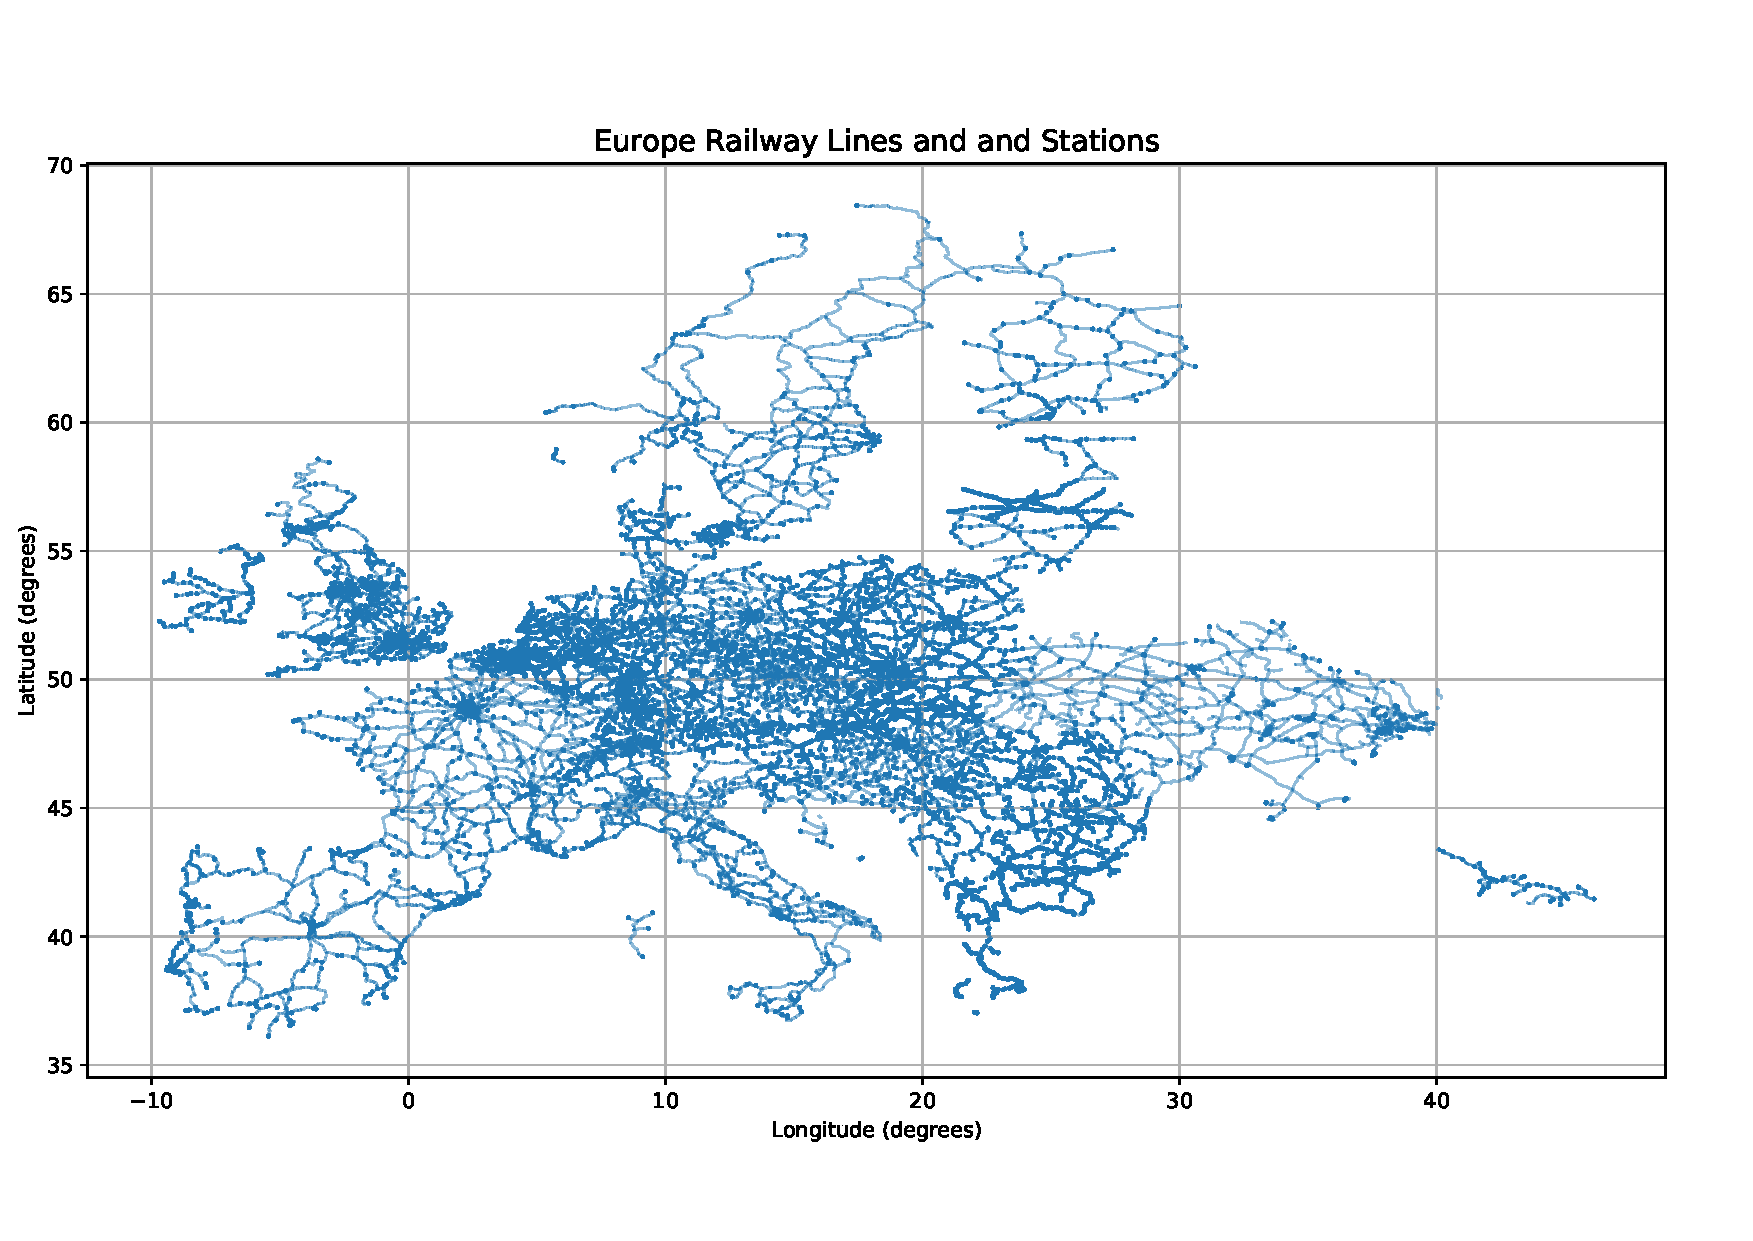
\includegraphics[width = 0.8 \textwidth]{latex_source/images/railways/europe.pdf}
    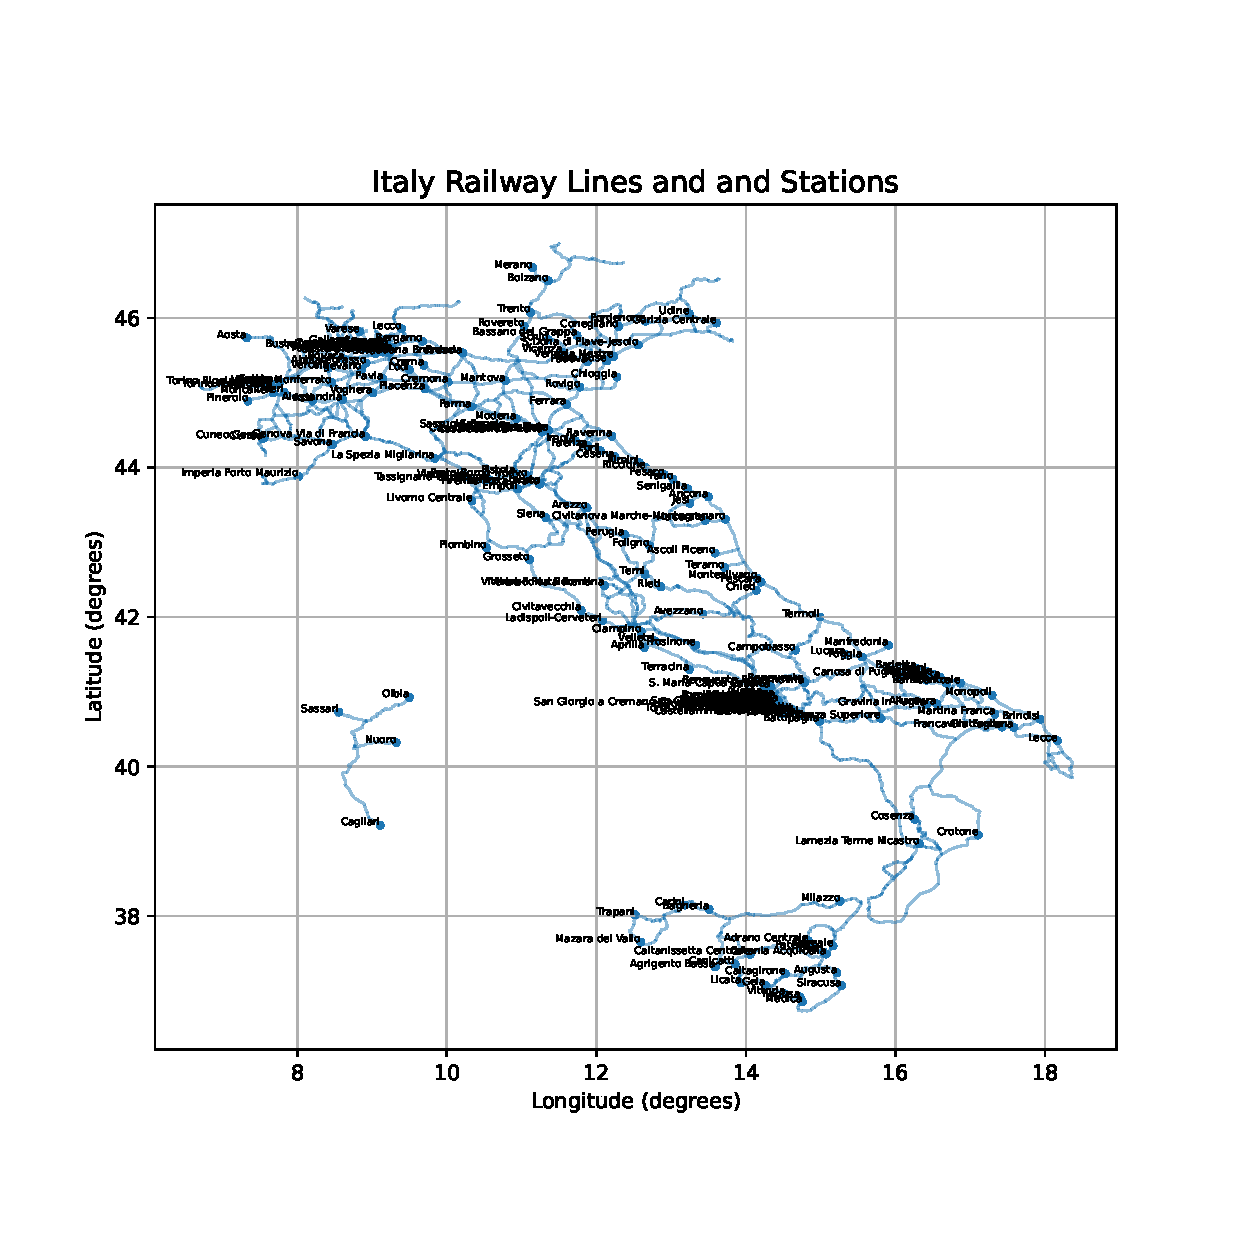
\includegraphics[width = 0.7\textwidth]{latex_source/images/railways/italy.pdf}
    \caption{\textbf{Top}: Railways and stations of the whole Europe. Each dot (line, respectively) is an element of the dataframe stations (railways, respectively). Only operational lines (EXS code $= 28$) have been filtered out. \textbf{Bottom}: A zoom on Italy. We can already see by eye that data is incomplete (for instance,stations of Verona, Trieste and Roma are missing form the chart). Also, in the metropolitan area of Napoli there is a high density of stations, because also the smallest ones are reported in the database, whereas for other areas of Italy (like Veneto) only the biggest stations are reported. We cannot thus expect to recover a very accurate network of railways from this dataset.}
\end{figure}

\section{Creation of the "raw" networks}
To create the raw graph we used Python library \textbf{NetworkX}. 
In the raw graph, each straight segment of rails, corresponding to two consecutive items in a LineString object, is assigned to an edge. The starting point and ending point of the segment are assigned to nodes. Identifiers of nodes are sequential integer numbers starting from $1$. A helper function \textbf{add\_node} is defined to handle node numbering properly and avoid adding the same node to the graph more than once (which, anyway, seems unlikely having such high precision on coordinates... but never say never!).

Finally, the graph data is stored as node list with attributes \textbf{"{ICC}\_raw\_nodes.csv"} and edge list \textbf{"{ICC}\_raw\_edges.csv"}
via basic networkx and pandas methods.


\section{Creation of the city/railways networks}
The creation of the raw network was straightforward; however, the refined network required a few specific steps:
\begin{enumerate}
\item Data was read from "RailrdC.shp" to create a list of city nodes\textbf{"{ICC}\_city\_nodes.csv"}. This file contains the columns: nodeID, nodeLabel, latitude, longitude, country\_name, and country\_ISO3.
\item The raw graph data "{ICC}\_raw\_nodes.csv" and "{ICC}\_raw\_edges.csv" is recovered. Attributes 'label' and 'is near city' are added to raw nodes. A raw node that matches a city's coordinates in "{ICC}\_city\_nodes.csv" within a specified threshold distance was assigned either "label" = "city\_name" and "is\_near\_city" = "empty" (if it was the best match) or "label" = "empty" and "is\_near\_city" = "city\_name".
\item The city/rails graph was derived as a subset of the current graph: for each pair of labeled nodes ('label' $\neq$ 'empty') that are within a maximum radius, the shortest paths were calculated. If a shortest path existed where all intermediate nodes were neither cities nor dangerously close to other cities, an edge was added to the final output graph.
\end{enumerate}
Then, the graph is created and saved with usual routines. Final output files are \textbf{"{ICC}\_nodes.csv"} and \textbf{"{ICC}\_nodes.csv"}.
\medskip \newline
The introduction of the "is\_near\_city" field was necessary because rail bifurcations often start slightly before or after entering a city station. In reality, the train must pass through the city station even if it takes the bifurcation. Without the "is\_near\_city" field, non-existent edges would be erroneously created (see figure \ref{fig:pescara_area}). The maximum radius parameter for checking edges only between sufficiently close cities was crucial for speeding up computations, especially in countries with a high number of stations and densely connected railways, such as Poland. Both threshold parameter for city matching in \textbf{flexible\_matching} and maximum radius have to be tuned after looking at the raw data.
\begin{figure}[H]
    \centering
    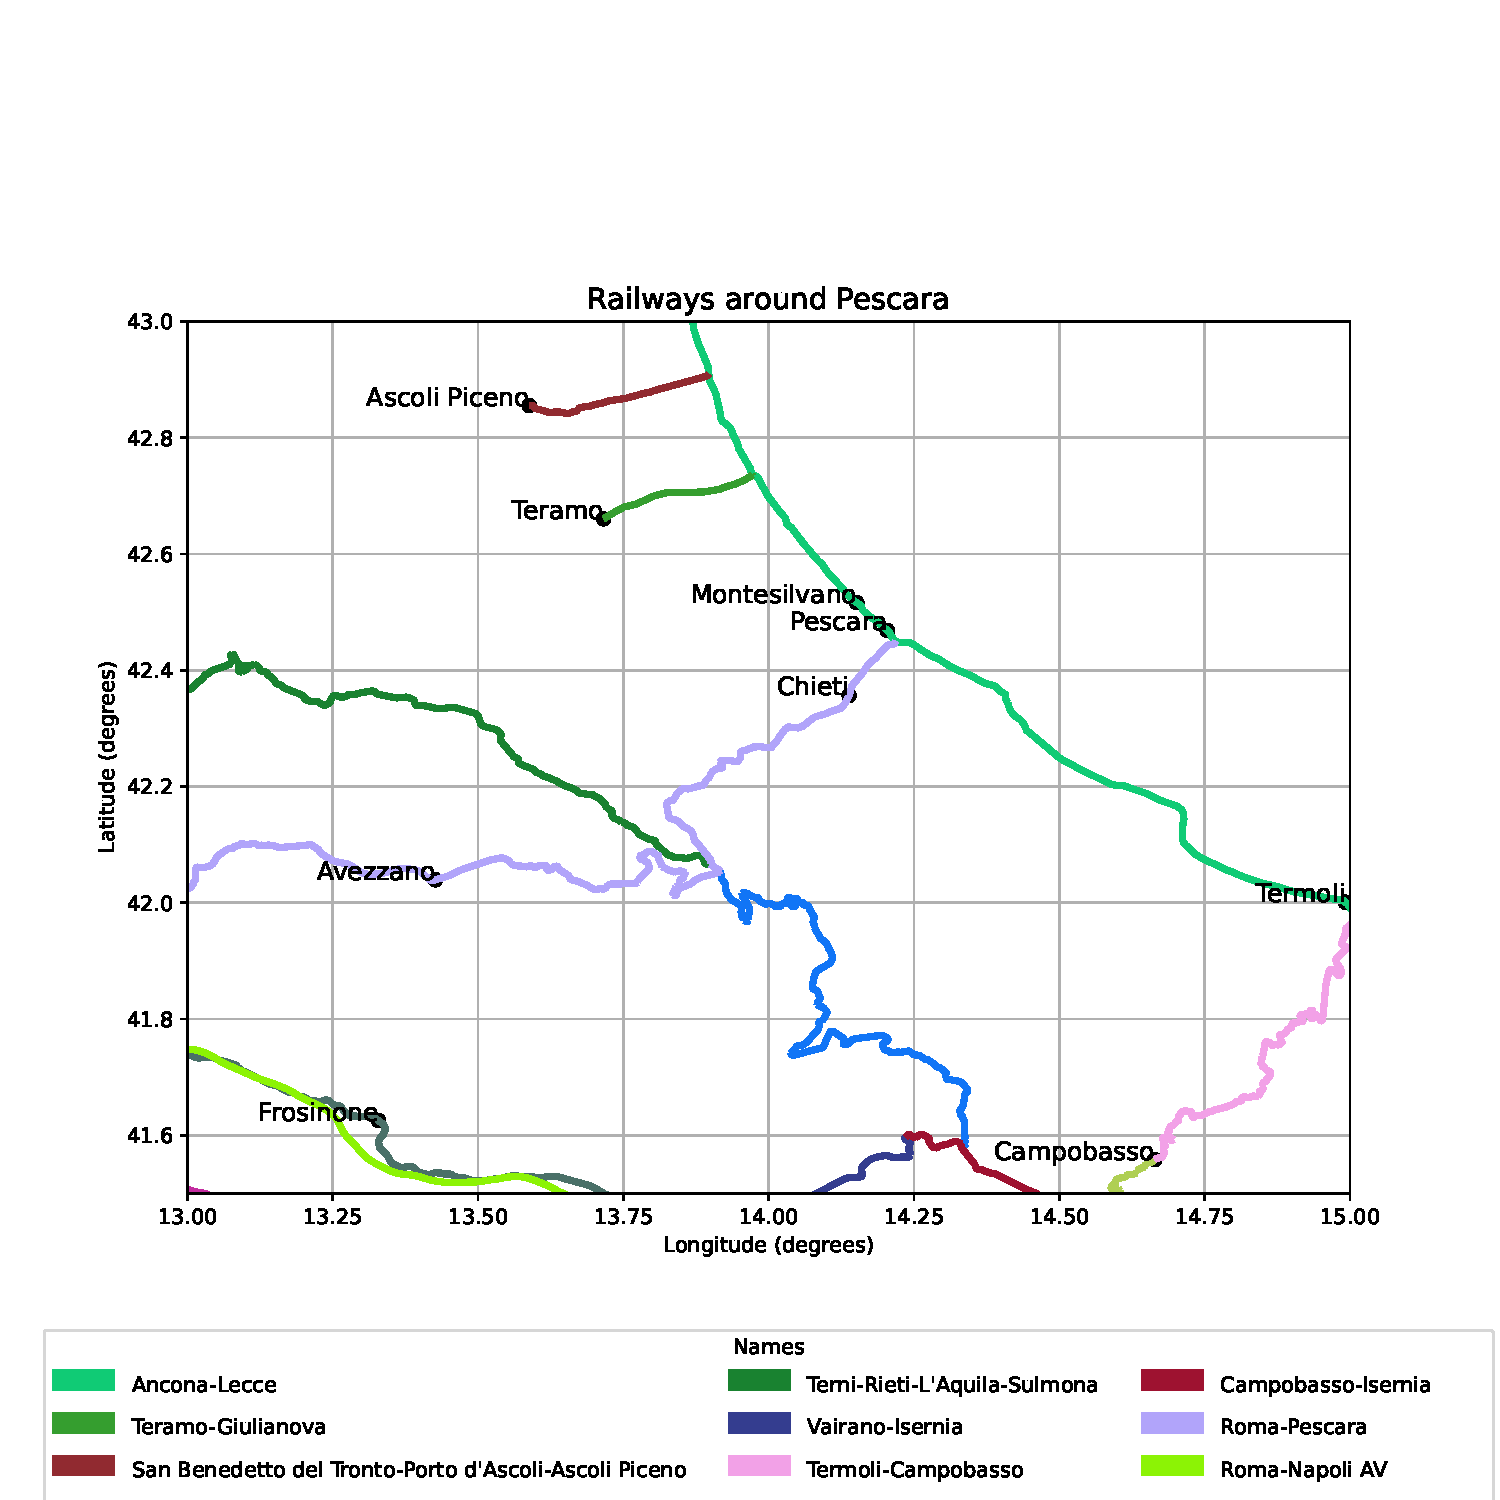
\includegraphics[width= \textwidth]{latex_source/images/railways/pescara_area.pdf}
    \caption{An example to justify the need for the "is near city" check: a rail bifurcation starts just before entering Pescara from south. Without the check implementation, edge "Termoli-Chieti" is created whereas in reality it does not exist: one wanting to get to Chieti must first get to Pescara, then take another train to Chieti. }
    \label{fig:pescara_area}
\end{figure}
\newpage
\section{Results Visualization}
\begin{figure}[H]
\centering
    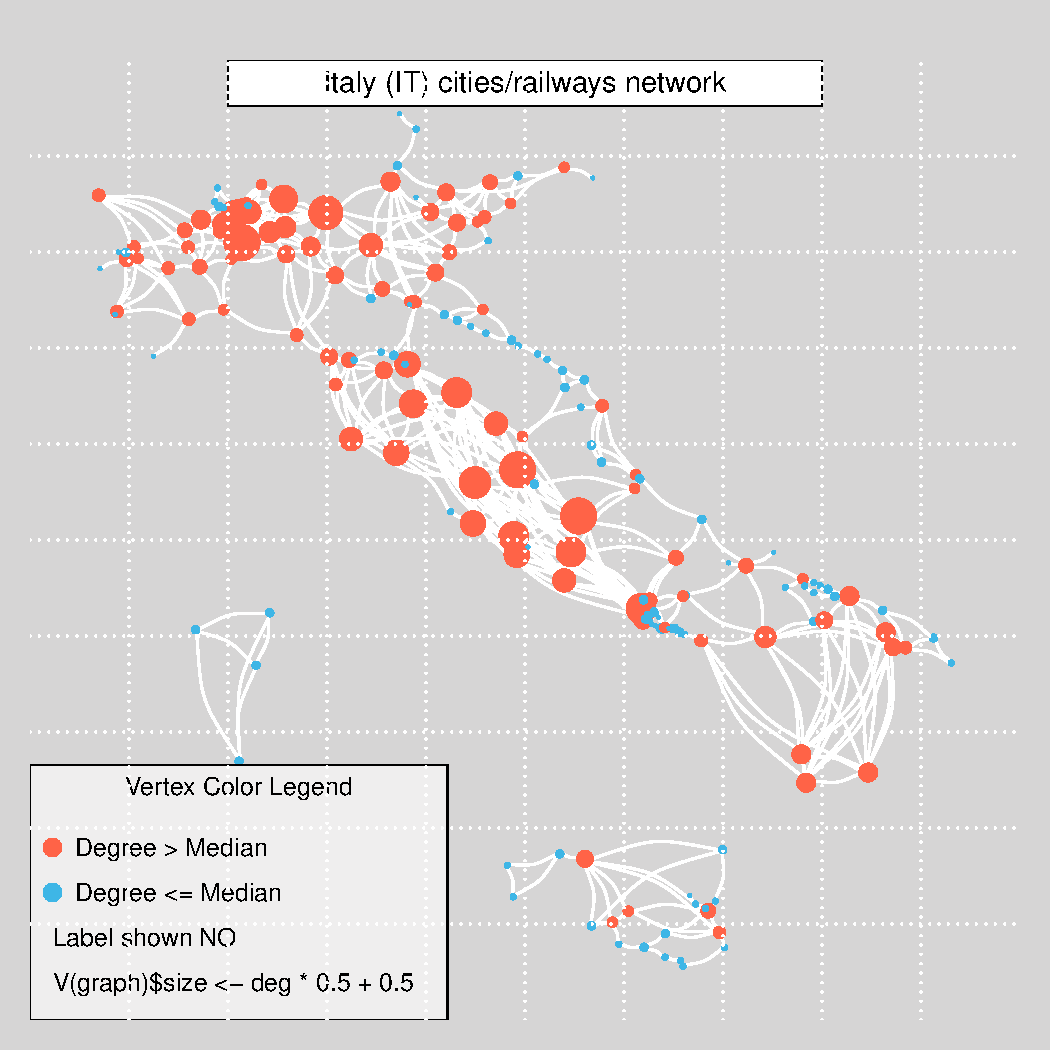
\includegraphics[width = 0.7\textwidth]{latex_source/images/railways/city_networks/IT_network.pdf}
\begin{comment}
IT (Italy) cities/ railways networks. Note the high density of edges in the center-left zone of the graph: it is a consequence of the fact that the stations "Roma Termini" and "Roma Tiburtina" are missing from file "RailrdC.shp". Many stations result directedly connected where in reality they are not because Rome stations are in between.
\end{comment}

\begin{subfigure}{}
    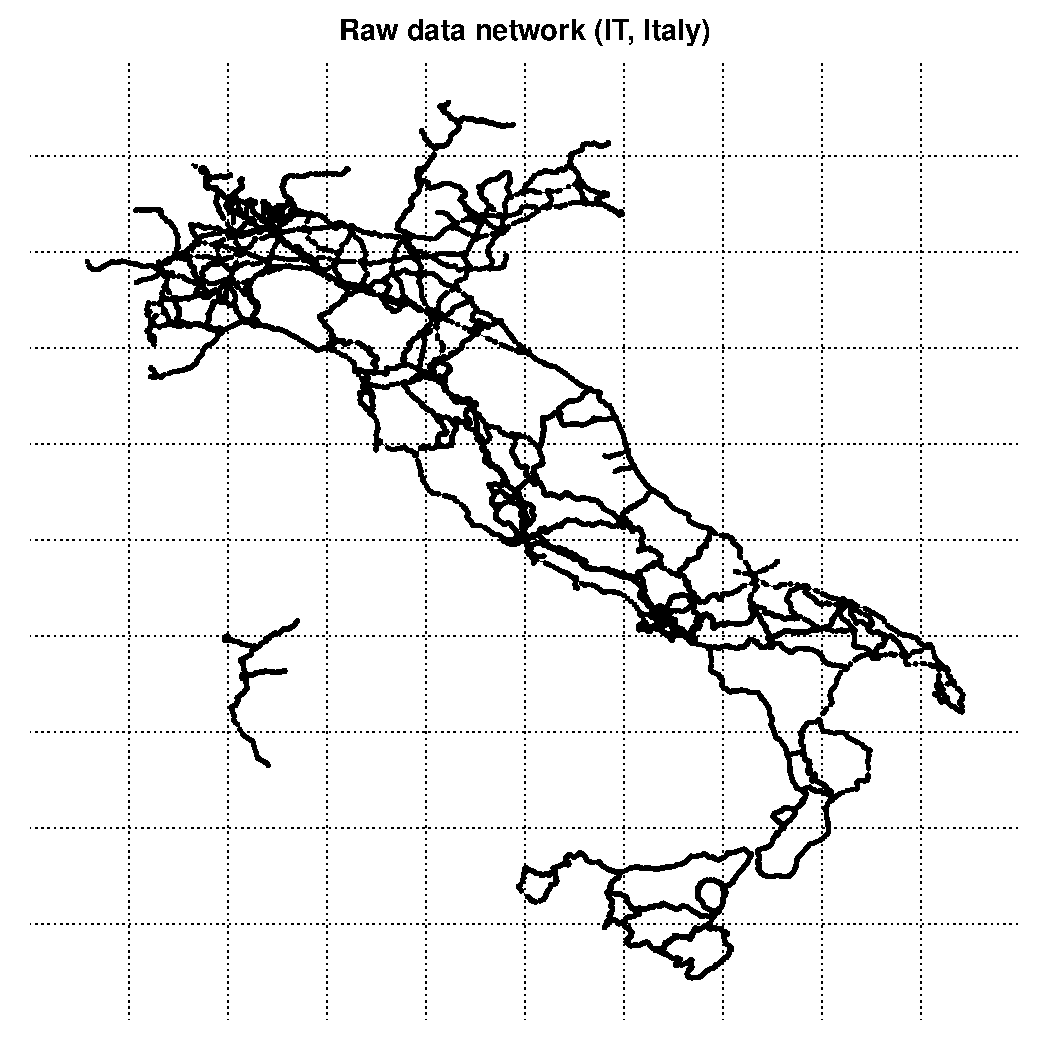
\includegraphics[width = 0.3\textwidth]{latex_source/images/railways/raw_networks/raw_IT_network.pdf}
\end{subfigure}
\begin{subfigure}{}
    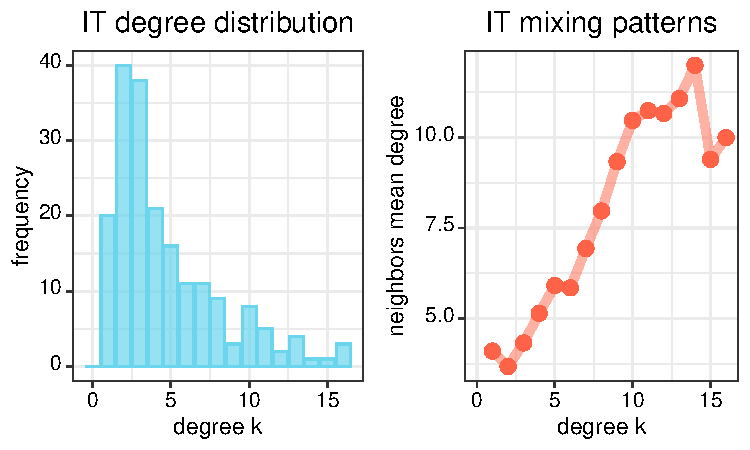
\includegraphics[width = 0.6\textwidth]{latex_source/images/railways/city_network_analysis/IT_analysis.pdf}
\end{subfigure}
\caption{}
\end{figure}
\newpage